%& C:\Users\RANGAR~1\AppData\Roaming\TikzEdt\TikzEdt\023~1.0\TEMP_H~1
\begin{document}
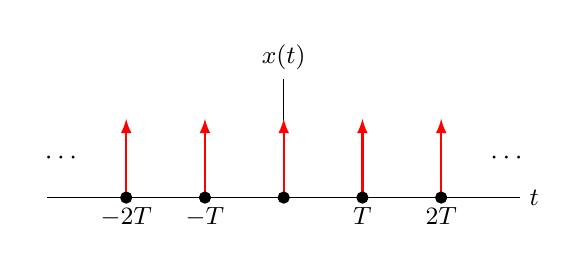
\begin{tikzpicture}
	\def\w{{-2, -1, 0, 1, 2}}
	\def\akmag{{1, 1, 1, 1, 1}}


	\begin{scope}	
		\draw (-3, 0) -- (3,0) node[anchor=west] {\small $t$};
		\draw (0, 0) -- (0,1.5) node[anchor=south] {\small $x(t)$};		
		\foreach \k/\l in {-2/{-2T}, -1/{-T}, 0/{}, 1/{T}, 2/{2T},}
		{
			\node at (\k, 0) [anchor=north] {\small $\l$};
		}
		%\node at (0,5) [anchor=south] {\small $Ta_k$};
		
		\foreach \k in {0,1, ..., 4}
		{
			\pgfmathparse{\w[\k]}
			\edef\wk{\pgfmathresult}
			\pgfmathparse{\akmag[\k]}
			\edef\akmagk{\pgfmathresult}	
			\draw[thick, red, -latex] (\wk, 0) -- ++(0,\akmagk);% node [anchor=south] {\small $\akmagk$};
			\ifthenelse{\lengthtest{0 pt = \akmagk pt}}{\draw[fill=black]  (\wk,0) circle (2pt);}{}
		}
			\node at (2.5, 0.5) [anchor=west] {$\cdots$};		
			\node at (-2.5, 0.5) [anchor=east] {$\cdots$};					
	\end{scope}
	
\usetikzlibrary{calc}
\pgftransformreset
\node[inner sep=0pt,outer sep=0pt,minimum size=0pt,line width=0pt,text width=0pt,text height=0pt] at (current bounding box) {};
%add border to avoid cropping by pdflibnet
\foreach \border in {0.1}
  \useasboundingbox (current bounding box.south west)+(-\border,-\border) rectangle (current bounding box.north east)+(\border,\border);
\newwrite\metadatafile
\immediate\openout\metadatafile=\jobname_BB.txt
\path
  let
    \p1=(current bounding box.south west),
    \p2=(current bounding box.north east)
  in
  node[inner sep=0pt,outer sep=0pt,minimum size=0pt,line width=0pt,text width=0pt,text height=0pt,draw=white] at (current bounding box) {
\immediate\write\metadatafile{\p1,\p2}
};
\immediate\closeout\metadatafile
\end{tikzpicture} 

\end{document}

